\documentclass{article}
\usepackage{tikz}
\usetikzlibrary{calc}

\newcommand*{\GridSize}{4}

\newcommand*{\ColorCells}[1]{% #1 = list of x/y/color
  \foreach \x/\y/\color in {#1} {
    \node [fill=\color, draw=none, thick, minimum size=1cm] 
      at (\x-.5,\GridSize+0.5-\y) {};
    }%
}%


\begin{document}

\section{Part 0.2}
$\sqrt{1+2\sqrt{1+3\sqrt{1+4\sqrt{1+...}}}} = \sqrt{2}^{\sqrt{2}^{\sqrt{2}^{\sqrt{2}...}}}$

$\newline$

\section{Part 0.3}
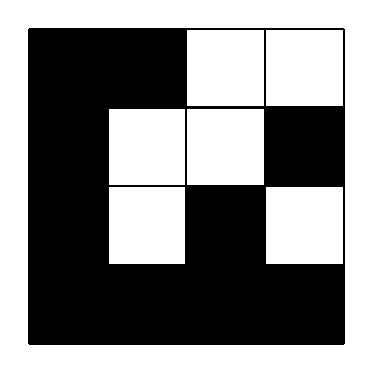
\begin{tikzpicture}[scale=1]

    \begin{scope}[thick,local bounding box=name]
        \ColorCells{1/1/black, 1/2/black, 1/3/black, 1/4/black, 2/1/black, 2/4/black, 3/3/black, 3/4/black, 4/2/black, 4/4/black}
        \draw (0, 0) grid (\GridSize, \GridSize);
    \end{scope}


\end{tikzpicture}

\end{document}